\chapter{Analogue to Digital Converter}
\section{Functional Theory}
Before discussing an Analogue to Digital Converter (ADC), first consider the simple GPIO pin configured as an input. 
The pin `reads' the voltage applied to it and produces a binary number (a 1 or a 0) which indicates whether the applied voltage is a high or low. Technically this GPIO pin is an analogue to digital converter: it takes an analogue voltage and produces a binary number.
However, having only 1 bit to represent the voltage applied to the pin means that we get a very poor approximation of the voltage. For example, we cannot tell the different between 2 V and 3 V being applied to the pin: both of those voltages are considered a logic 1. 
For this reason we do not typically refer to a GPIO pin as an ADC, rather we refer to it as a digital input.

The term ADC is typically reserved for a peripheral inside the microcontroller which has the ability to provide a much higher resolution and higher accuracy numerical approximation of the applied voltage. 
While a GPIO pin is able to digitise the voltage to only 1 bit, the ADC can digitise the voltage to many bits. 

\begin{table}[t]
\centering
\begin{tabu}{c | l}
    Output & Voltage Band (V)\\
      \hline
      00 & 0.00 - 0.75\\
      01 & 0.75 - 1.50 \\
      01 & 1.50 - 2.25 \\
      11 & 2.25 - 3.00 \\
\end{tabu}
\caption{Numerical output vs applied voltage band for a 2 bit ADC running off of 3 V}
\label{tab:2_bit_ADC}
\end{table}

The number of bits determines the number of \emph{quantization levels} which the system has. Quantisation levels are the voltage bands which the digitiser produces. 
Consider the trivial case: a GPIO pin. This digitises to 1 bit, and hence has $2^1 = 2$ quantisation levels. Specifically: a logic high or a logic low.
If we consider a system running off of a 3 V supply rail, the two levels would be 0 V to 1.5 V and 1.5 V to 3 V\footnote{Actually, a GPIO pin is more complicated due to its hysteresis which defines different levels for high-to-low or low-to-high transitions.}. If the applied voltage is between 0 V and 1.5 V the digitiser will produce an output of 0. If the applied voltage is between 1.5 V and 3 V the digitiser will produce a logic 1. Clearly the `size' of each quantisation level is equal to $\frac{V}{N} = \frac{3}{2} = $ 1.5 V \\

Now consider the case where we have an ADC which can produce 2 bits of output. Here we will have $2^2 = 4$ quantisation levels. The size of each level will be $\frac{V}{N} = \frac{3}{4} =$ = 0.75 V. The relationship between digital output and applied voltage can be seen in \autoref{tab:2_bit_ADC}.


From these two simple examples we start to build up a picture of how the ADC relates applied voltage to numerical output:
\begin{itemize}
\item The supply rail is divided up into $N = 2^M$ levels, where $M$ is the number of bits of the ADC.
\item Each quantisation level has a range of $Q = \frac{V}{N}$ volts.
\item The start of level $k$ is equal to $k \times Q$ where $k$ is some number produced by the ADC.
\item The end of level $k$ is equal to the start of the next level, or: $(k+1) \times Q$.
\item An applied voltage $v$ will produce a numerical output of $\lfloor v \div Q \rfloor $.\footnote{The `$\lfloor$' and `$\rfloor$' symbols mean `floor'. In other words: round down to the nearest integer.} This essentially says: "We know each level is $Q$ voltage wide. How many levels up must we go to get to voltage $v$?"
\end{itemize}

That concludes the overview of what an ADC is and how it relates applied voltage to numerical output. We will now consider how to configure and use the ADC on our STM32.

\section{Using the ADC}
\subsection{Enabling}
Before the ADC peripheral can be used, it should be enabled. Two steps are required: 
\begin{enumerate}
\item Externally activating the ADC by providing clock to the peripheral by setting the corresponding bit in the RCC\_APB2ENR
\item Internally activating the ADC by setting the ADEN bit in the ADC\_CR
\end{enumerate}

After setting the ADEN bit, the ADC will take some time to power on. Once the ADEN bit has been set, you should wait until the ADRDY flag in the ADC\_ISR has gone high before you attempt to do anything with the ADC. 

\subsection{Channel}
The ADC is not limited to just reading from one fixed pin; it can select which pin to use from a number of possible sources, or \emph{channels}.
The ADC\_CHSELR register controls which channel is selected. On our device there are 10 different pins which can be selected for use as an ADC channel. In order to see which ADC channel a pin corresponds to, consult Table 13 of the Datasheet. This table shows which ADC channel a pin is connected to in the `Additional functions' column. For example, PB1 is connected to ADC channel 9.

Be careful not to set multiple channels in the ADC\_CHSELR simultaneously. If you do this, the ADC will scan through each of the channels. Unless you know what you're doing, this is probably not what you want and it will confuse you.

\subsection{Pin Mode}
We know that by default a pin will operate in \emph{Input} mode. That is, it will digitise the applied voltage to a 1 bit number which will set/clear a bit in the GPIOx\_IDR. The component which does the digitising is the Schmitt trigger. 

This is now how we want the pin to function when using an ADC. When we want to use a pin as an ADC channel, we want the raw analogue voltage to be passed on to the ADC for digitising. In order to achieve this, the pin should be put into \emph{Analogue} mode. Here, the Schmitt trigger is disabled and the pin is made accessible to analogue peripherals (such as the ADC). The structure of a pin in analogue mode can be seen in \autoref{fig:pin_analogue_mode}. Note the top of the diagram where it can clearly be seen that the raw analogue voltage is sent off to the ADC peripheral.

\begin{figure}
\centering
\includegraphics[page=158, clip=true, trim=130 150 70 480, width=\textwidth]{./stm32f0xx_reference_manual}
% left, bottom, right, top
\caption{Structure of pin in Analogue mode. Source: Figure 21, Reference Manual}
\label{fig:pin_analogue_mode}
\end{figure}

In order to set a pin to operate in analogue mode, both both bits which control that pin in the GPIOx\_MODER should be set to 1. See Section 9.4.1 of the Reference Manual for more info on the modes. 

\emph{Be very careful when setting the modes of Port A pins. Remember that PA14 and PA13 are Alternate Function by default and must remain so for debugging to work.}


\subsection{Resolution and Alignment}
Our ADC can operate in one of 4 different resolutions: 6-bit, 8-bit, 10-bit or 12-bit. The resolutions which it will use is set by the RES bits in the ADC\_CFGR1. A higher resolution allows a better approximation of the real applied voltage, while a lower resolution will allow the ADC to perform the conversions faster as it has less work to do.

The numerical output of the ADC is made available in the ADC\_DR (data register). This register is 16 bits wide. So, how will the result of the ADC conversion (which is less than 16 bits) be presented in the ADC\_DR? This is a question of data alignment and is controlled by the ALIGN bit in the ADC\_CFGR1. The structure of the ADC\_DR for all combinations of resolution and alignment is shown in \autoref{fig:adc_res_align}. Which one should you use? Depends entirely on your application. 

\begin{figure}
\centering
\includegraphics[page=220, clip=true, trim=70 440 70 250, width=\textwidth]{./stm32f0xx_reference_manual}
% left, bottom, right, top
\caption{Structure of data in ADC\_DR for combinations of resolution and alignment. Source: Figure 36, Reference Manual}
\label{fig:adc_res_align}
\end{figure}

\subsection{Performing Conversions}
A conversion is the name for the process when the ADC reads the voltage and \emph{converts} it into an equivalent number.
Once the ADC has been enabled and the channel, resolution and alignment selected the ADC can start doing conversions. As mentioned earlier, the conversions take some time to complete. This is due to the nature of the architecture of the ADC. Our ADC is a successive approximation (SAR) ADC which means that it progressively narrows down the numerical representation of the voltage to the final output by using a binary search. A full understanding of how a SAR ADC works is outside the scope of this course, but for those interested there is a good wikipedia article on it: \url{https://en.wikipedia.org/wiki/Successive_approximation_ADC}. 

Suffice to say, from the moment that you tell the ADC to read the voltage (start a conversion) until the data is ready, there is some delay. This delay varies with ADC resolution and clock scheme, but it's typically in the order of a microsecond. This means that you cannot read the result of the conversion immediately from the ADC\_DR. Instead, you should wait until the ADC signals it has finished the conversion. This is done by waiting for the EOC flag in the ADC\_ISR to go high. The process is as follows:
\begin{enumerate}
\item Start a conversion by setting the ADSTART bit in the ADC\_CR
\item Wait for the EOC bit in the ADC\_ISR to go high
\item Read the result from the ADC\_DR. The result is in a format as defined by the resolution and alignment. 
\end{enumerate}
Note that by reading from the ADC\_DR the EOC flag is automatically cleared. If you do not read the contents of the ADC\_DR the EOC flag will not be cleared which may cause issues the next time to start a conversion. 



